\section{Caching and acceleration} 
\label{sec:caching}

As NVMM outperform traditional storage devices with low latency and high
bandwidth, build a persistent cache for slower storage devices and
accelerate the file access is a good usage of NVMM. 

\textbf{Rio}~\cite{riofilecache} uses battery-backed memory to build a
operating system
with better performance and able to recovery from crash. Rio stores regular
files in the unified buffer cache on the NVMM, and recover the files
during system recovery.
To prevent the file
cache from corrupt during system failure, Rio turns off the write-permission
bits in the page table for all file cache pages, only enable it during page
writing. Rio also disables the ability of the processor to bypass the TLB,
enforce the protection for all the pages. With these mechanisms, Rio guarantees
that the file cache will not be accidentally overwritten by the system during
a crash.

Rio uses the warm reboot mechanism to rebuild the system. When the system 
recovers from failure, it read the file cache extents present in physical memory
and update file system with the data. To figure out the file cache contents,
Rio also needs to store the metadata for the file cache. Rio allocates a
separate region of memory called registry to store the metadata information.
This makes Rio looks like a NVMM file system.
To minimize the software changes, Rio first dump the file cache to swap
partition, and then use a user-level process to analyze the memory dump
and restores the file cache.

Rio improves the system performance by eliminating the sync and fsync system
calls, which are expensive in the original system. However, as buffer cache
is persistent now, the write ordering is essential to make sure the system
works correctly. Rio does not explain how it works on write ordering and CPU
caching impacts.

Another contribution of Rio is that it proposes several fault models of system
failure to memory and tested the system with thousands of reboot. This makes
it more reliable.
 
\textbf{Rio Vista}~\cite{riovista} is a combination of RVM and Rio.
It is an evolutionarywork of Rio, and relate closely to RVM design.
Like RVM, Rio Vista is a
user-level, recoverable-memory library, and it runs on Rio. Unlike RVM,
which has undo log and redo log, Rio Vista just has one undo log. When
application starts a transcation, Rio Vista copies the origial data to the 
undo log, which is kept in NVMM provided by Rio, and then application can
write new data in-place and discards the undo log by the end of the transaction.

Rio Vista is trying to be simple, handles only the basic transaction features
of atomicity and persistency. Like Rio, it does not address the write ordering
issue and CPU caching issue, which undermines its credability. 

\textbf{Chell}~\cite{Chell} is the system we built that accelerate storage
access with NVMM. Chell can be configured to work in two modes: \DAChell{}
and \CChell{}. \DAChell{} accelerates access to files stored in file systems
that reside solely in NVMM, while \CChell{} uses NVMM as a cache for the
slower storage devices. Below we describe the architecture and implementation
of \DAChell{} and \CChell{}.

\subsection{\DAChell{}}

\cfigure[Figures/ChellD-Stack.pdf,{\figtitle{\DAChell{} architecture}: by combining NVMM with the ability to map files into userspace, \DAChell{} provides applications with a fast, POSIX-compliant interface to data stored in NVMM.},fig:dachell]


\DAChell{} works with a NVMM file system, gives applications direct access to
a file's contents without
requiring any interaction with the operating system in the common case.  As a
result, it can eliminate both the system call overhead required to enter the
kernel and the file system overhead required to locate stored data and perform
permission checks.
Figure~\ref{fig:dachell} shows the high-level architecture of
\DAChell{}. An NVMM-aware file system (e.g.,
PMFS~\cite{PMFS}) manages the NVMM space and allows users to create and manage
files that reside in the NVMM.

\DAChell{} is implemented as an user space library, \libd{}, that transparently 
link into application with LD\_PRELOAD and interposes on file access system
calls.
\DAChell{} exploits DAX \texttt{mmap()} to make common-case access to file data
fast.  When an application opens a file, \DAChell{} intercedes, and
\texttt{mmap()}s the file's contents into the application's address space.
This provides direct access to the file's data and transfers the permission and
extent information from the file system's data structures into the
application's page table, leveraging the processor's fast memory
protection hardware to locate the file's data and protect its contents.

When the application calls \texttt{read()} and \texttt{write()}, \DAChell{}
translates them into calls to \texttt{memcpy()} to transfer data between
application buffers and the memory mapped file.  Other operations such as
\texttt{lseek()} simply update the state (e.g., the current file pointer) that
\DAChell{} maintains about each open file.  Consequently, common-case accesses
require no calls to the operating system, avoiding costly system calls and 
operating system and file system overheads.

\DAChell{} cannot eliminate all interactions with the operating system.  In
particular, any operations that modify file system meta data still must enter
the OS.  This means that \DAChell{} helps performance less for appends than for
normal write operations, since it needs to make a system call to extend both
the file and the in-memory mapping.  
Also, the updates to the file's modification time do not occur as they
would with normal accesses.  However, many performance-intensive applications
already disable file modification and access time updates to improve
performance.

\DAChell{} divides file into 2MB chunks as \texttt{mmap()} unit. This
reduces the number of \texttt{mmap()} operations, and perform well as 
a prefetch mechanism for small sequential requests.  
\DAChell{} issues \texttt{mmap()} with the MAP\_POPULATE flag set to force the
kernel to
populate the application's page table immediately and hence reduce page faults.
With micro- and macro-benchmark, We found that \DAChell{} improves 4~kB access
latency by up to 19\% relative to file access through a PMFS, and improves
Berkeley-DB performance by 6\% over PMFS.

\ignore{
Below we discuss the POSIX compatibility and implementation details of
\DAChell{}.

\subsection{POSIX Emulation}

\DAChell{} mimics the behavior of the normal POSIX file
interface. It also
enforce access restrictions (e.g., disallowing \texttt{write()} calls if the
file opened read-only, even if the file's permissions allow modification).
Implementing this functionality requires \DAChell{} to duplicate much of the
information that the kernel would usually manage.  This includes file
descriptor permission information, the close-on-exec flag, file position
information, and file descriptor aliasing information. For file descriptors
that point to files that don't reside in NVMM or that represent
network sockets and other resource, \DAChell{} passes requests to the default
POSIX functions that perform normal system calls.

\DAChell{} avoids the need to modify application source code or recompile by
using LD\_PRELOAD.  This allows \DAChell{} transparently link into the
applications and interpose on calls to libc.

\subsection{Implementation}

After the POSIX emulation determines which data an read or write targets, the
\DAChell{} translates the file operation into an operation on the memory mapped
contents of the file.

For each file being accessed via \DAChell{}, \DAChell{} divides the file into
2~MB \emph{chunks}.  A B-tree store information about the file's
\texttt{mmap()ed} chunks.  The key is the file offset, and the value is the
mapped address and length.  For each access, \DAChell{} queries the tree for
the mapping information.  If it finds the data, it performs a \texttt{memcpy()}
to transfer data between application buffers and the memory mapped NVMM pages.

If the file offset is not present in the B-tree, \DAChell{} uses
\texttt{mmap()} to map the data into the application's addresss space. Then,
it updates the B-tree and performs the \texttt{memcpy}.

\DAChell{} \texttt{mmap()s} 2~MB at a time, because \texttt{mmap()} is expensive
and when the file size changes, it may be necessary to remap the entire file. 
Mapping two megabyte chunks amortizes the cost of mapping and reduces the need
for remapping.  It also limits the number of memory-mapped regions the kernel
must maintain. Each \texttt{mmap()} request allocates a
virtual memory area (vma) in application's address space, and Linux kernel
limits each process to have up to 65,536 vmas. If the requests are small and
frequent, \texttt{mmap()}ing each of them will exhaust this number very quickly.
For small requests, the 2~MB \texttt{mmap()} also works as a prefetching
mechanism, reduce the overhead for small sequential requests.

\DAChell{} issues \texttt{mmap()} with the MAP\_POPULATE flag set to force the kernel to
populate the application's page table immediately.  Without the flag, the first
access to each page causes a page fault, degrading performance.

\DAChell{} relies on the DAX-style behavior of \texttt{mmap()} that maps NVMM
directly into the application's address space.  DAX-like functionality has
existed in some file systems for many years.  It used to be called
\emph{eXecute In Place}, or XIP, and mostly found use in embedded systems that
needed to execute
code directly from NOR flash devices.  DAX capabilities are already present in
PMFS~\cite{PMFS} and efforts are underway to add it to other file sysetms~\cite{ext4dax}.

With micro- and macro-benchmark, We found that \DAChell{} improves 4~kB access
latency by up to 19\% relative to file access through a PMFS, and improves
Berkeley-DB performance by 6\% over PMFS.
}

\subsection{\CChell{}: Accelerating Legacy Storage with NVMM}
\label{sec:overview}

\DAChell{} is useful if the entire file system resides in NVMM, but many
storage systems are too large to fit in NVMM.  To improve
performance of these systems, \Chell{} provides an alternative mode of
operation called \CChell{}.  \CChell{} uses NVMM to provide a reliable,
consistent, write-back cache of data that resides in an existing file system.
\CChell{} provides fast access to the cached data using the same techniques
that \DAChell{} uses but it accesses cached data rather than actual file data.
This section describes the differences between \CChell{}
and \DAChell{}.

Figure~\ref{fig:CChellstack} shows the system architecture of \CChell{}.
Like \DAChell{}, there is an userspace library, \lib{} to handle cache
hits, but \CChell{} also adds a kernel module, \drv{}, to
manage the contents of the cache and interact with the file system on the
backing store device.

The only difference in \libd{} and \lib{} is in
how they detect and react to a miss.  \Libd{} detects a miss when it
finds that the request region is not mapped, and it 
issues an \texttt{mmap()} to map the chunk. When
\Lib{} experiences a miss,
it issues an \texttt{ioctl()} to \drv{} requesting that
it load the data from the backing store (if needed), and then map the data into
the application's address space.

\Drv{} manages the data cached in the NVMM.
It copies data between cache pages and the backing store device,
memory maps the requested cache pages to the application's address space,
and handles cache write back and eviction.

When \drv{} receives the \texttt{ioctl} request from \lib{},
it first checks the
file Inode permission to make sure it is a valid request.  Then it checks if 
the requested data is in the cache,
and loads it, if required.
Next, \drv{} copies data from the user buffer to the cache pages if it is
a write, or from the backing store device to the cache pages and user buffer if 
it is a read. Then it calls \texttt{mmap()} to map the cache pages to
the application's address space and returns the mapped address and length
to \lib{}.

%\cfigure[Figures/Chell-Stack.pdf,{\figtitle{\CChell{} system stack}},fig:CChellstack]

\begin{figure}
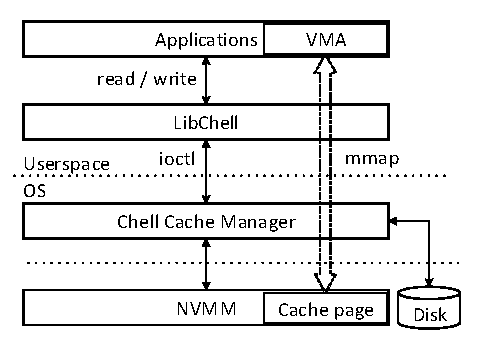
\includegraphics{Figures/Chell-Stack.pdf}
\caption{\CChell{} architecture: \CChell{} caches files stored on slow storage
devices in NVMM, provides a fast, POSIX-compliant interface to applications.}
\label{fig:CChellstack}
\end{figure}

\ignore{
By default \CChell{} requires all the applications to access the NVMM cache via
\lib{}.  Otherwise, if one application accesses a cached file via \CChell{}, while another
application accesses the same file on the backing store device via POSIX write,
\CChell{} and the file system on the backing store device will have an
inconsistent view about the file.  To prevent this inconsistency, \drv{}
interposes at the block device driver for the backing store and rejects
accesses that touch cached data but that are not from applications using \lib{}.

The space allocation and management system in \drv{} is based on PMFS.  It
allocates NVMM in 4~kB pages to minimize fragmentation and wasted space for
small files.  For file systems that store mostly large file, larger 2~MB or
1~GB pages would improve
TLB performance, reduce the number of page faults, and shrink the page table.

\CChell supports DAX interface for \texttt{mmap()} operation.
The cache page will be mapped directly to the application's
address space and avoids the overhead of the page cache and the block layer
for normal \texttt{mmap()} operations.
}
Like \DAChell{}, \CChell{} divides the cached file into 2~MB chunks and
\texttt{mmap()} with 2~MB granularity.
\CChell{} uses LRU to decide which cache page to evict when the cache is full,
and undo logging to enure the cache metadata remains consistent in the event
of a crash.

\ignore{ 
Both \DAChell{} and \CChell uses \texttt{mmap()} to accelerate NVMM access.
Failure-atomic msync~\cite{atomicmsync} proposes a atomic commit of memory
pages change for \texttt{mmap()ed} files, by flushing memory pages to persistent
store first and then write back to the destination. For \DAChell{} and \CChell{}, as they are running on NVMM, there is no need to write back the data, and
\texttt{msync()} is simely a CPU cache flush.

When the cache is full and \drv{}
needs to evict cache pages, it needs to decide which cache pages to evict
and whether the cache pages are dirty. As \lib{} accesses the NVMM directly
on cache hits and \drv{} is unaware of many accesses to the cache data, this
becomes a challenge to \drv{}.

\drv{} maintains a LRU list of accessed files and always try to evict the least
recently accessed cache pages. Since we managed the LRU list as a queue,
the result is a blend of LRU and FIFO.
\CChell{} also leverages the virtual memory manager of operating system to
track the dirty cache pages. 
when a memory page is written, the hardware set the dirty bit in the 
page table entry (PTE) of the page. Before evicting a cache page,
\drv{} looks up the PTE in all the mappings of the page.  If
any PTE has its dirty bit set, \drv{} will write the cache page back to
backing store.

\CChell{} uses undo logging to ensure that the cache metadata remains
consistent in the event of a crash.  Whenever \drv{} needs to make
a change to a Cnode, allocate a Cnode, or re-allocate pages,
\drv{} records the data in the log and makes it persistent before writing
the new data in place.

Every metadata change is organized as a transaction.  \Drv{} starts
a transaction by allocating the required number of log entries in the journal.
Then, \drv{} fills the log entries with old metadata.
Each log entry is written to the journal and made persistent by flushing it
to NVMM before new data is written in-place.
After all the updates are finished, \drv{} commits the transaction
by writing a special ``finish'' log entry to the journal to invalidate the undo information.

If there is a power failure or system crashes, \drv{} can recover the cache
when the system reboots.  During recovery, \drv{} locates the log area using
the superblock,
identifies uncommitted transactions and applies the undo information in the log
to restore the metadata.
After all the uncommitted transactions have been undone, \CChell{} is in a
consistent state.
}

Evaluation result shows \CChell{} can
reduce 4~kB access latency by up to 50\% and improve Berkeley-DB performance
by up to 4.8\x{} relative to file access using the system's file buffer.
